\chapter{Results} \label{ch:results}

\section{Baseline Performance}

Table~\ref{tab:baseline-results} summarizes the baseline results for Qwen~2.5 7B-Instruct on BFCL~v4 simple\_python (400 test cases).

\begin{table}[h]
\centering
\caption{BFCL v4 Simple Function AST accuracy for Qwen~2.5 7B-Instruct across initial configurations.}
\label{tab:baseline-results}
\begin{tabular}{llrr}
\toprule
Config & Description & Correct & Accuracy \\
\midrule
B  & Raw model (no optimization)     & 6/400   & 1.5\% \\
PE & Few-shot prompting + guided      & 281/400 & 70.25\% \\
CD & Constrained decoding (guided)    & 291/400 & 72.75\% \\
\bottomrule
\end{tabular}
\end{table}

\noindent Without constrained decoding (Config~B), the model achieves only 1.5\% accuracy. The dominant failure mode is format non-compliance: 394 out of 400 outputs fail to parse as valid JSON, producing \texttt{Extra data} errors or empty results. The model is not incapable of understanding the queries---it simply cannot express its answers in the required structured format.

Constrained decoding (Config~CD) recovers 71.25 percentage points, achieving 72.75\% accuracy. Function selection reaches 100\% accuracy via \texttt{guided\_choice}, confirming that the format enforcement fully solves tool selection. The remaining 27.25\% failure rate is entirely in argument extraction: wrong numeric precision (e.g., 9.8 vs.\ 9.81), string format mismatches (e.g., ``kilometers/hour'' vs.\ ``km/h''), and incorrect optional parameter defaults.

Few-shot prompting (Config~PE) decreases accuracy by 2.5 percentage points relative to Config~CD. The three few-shot examples, targeting known failure modes, did not transfer across function domains. This negative result indicates that the argument extraction errors reflect the model's learned associations rather than a formatting gap that in-context examples can bridge.

\section{No-Training Methods}

The following configurations modify only the inference pipeline; model weights
are unchanged in all cases. Configs~CD and CD+Q establish the no-training
ceiling. Configs~PE, CD+Q+ITC, and CD+Q+RAG assess whether inference-time
interventions can improve on that ceiling.

\subsection{Constrained Decoding}

The two-stage constrained decoding pipeline eliminates the dominant failure mode
of Config~B. In the function selection stage, \texttt{guided\_choice} restricts
generation to the set of available function names: function selection accuracy
is 100\% across all 400 test cases, confirmed by inspection of the raw
prediction files. In the argument extraction stage, \texttt{guided\_json}
restricts generation to a JSON object conforming to the function schema,
ensuring that every output is structurally valid~\cite{willard2023efficient,
kwon2023vllm}.

The 27.25\% failure rate that remains after constrained decoding is entirely in
argument values. Four categories account for the observed failures: wrong
optional parameter defaults (e.g., \texttt{root\_type=''} where
\texttt{'all'} is expected), numeric precision errors (e.g., \texttt{9.8}
where \texttt{9.81} is expected), string format mismatches (e.g.,
\texttt{"kilometers/hour"} where \texttt{"km/h"} is expected), and location
format errors (e.g., \texttt{"New York"} where \texttt{"New York, NY"} is
expected). These failures share a common structure: the model's output is
semantically reasonable but does not match the specific convention that the
benchmark's ground truth encodes. Constrained decoding enforces structural
validity but cannot enforce semantic convention.

AWQ INT4 quantization reduces model memory from 14.25~GiB to 5.20~GiB (63.5\%
reduction) and inference startup time from 212~s to 35~s (83.5\% reduction),
with an accuracy change of $-0.5$~pp (289/400, 72.25\%)~\cite{lin2024awq}.
The failure distribution does not change: no new error categories are
introduced, and the relative frequency of existing failure types is unchanged.
The accuracy difference of two test cases falls within run-to-run variance,
confirmed by six re-runs that consistently produced 289/400. Config~CD+Q
therefore provides equivalent accuracy to Config~CD at a substantially
reduced memory footprint, and serves as the operating baseline for subsequent
no-training experiments. Fig.~\ref{fig:memory-accuracy} plots GPU memory
against accuracy for the main configurations.

\begin{figure}[htbp]
\centering
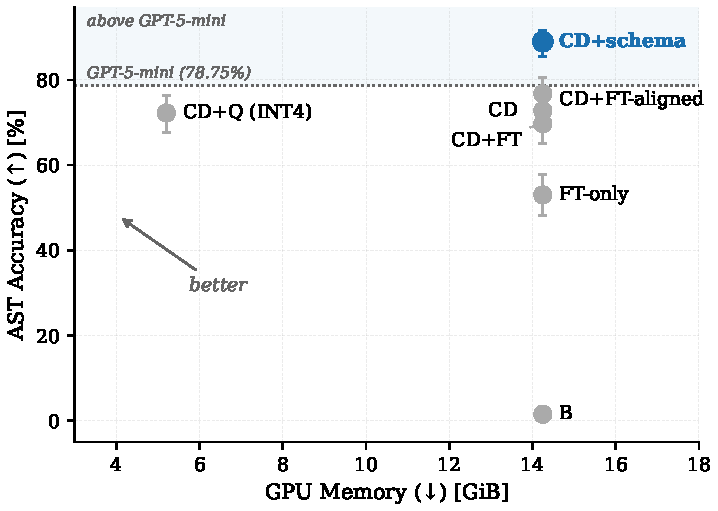
\includegraphics[width=0.65\textwidth]{pictures/figures/fig_memory_vs_accuracy.pdf}
\caption{GPU memory footprint vs.\ BFCL simple\_python AST accuracy for
         selected configurations. Config~CD+Q achieves equivalent accuracy
         to Config~CD at 63.5\% lower memory. The GPT-4.1 reference line
         (72.67\%) is shown for comparison.}
\label{fig:memory-accuracy}
\end{figure}

\subsection{Prompt Engineering and Few-Shot}

Three few-shot examples are prepended to the argument extraction prompt,
constructed to target the most frequent failure categories observed in
Config~CD: numeric precision (\texttt{9.81} rather than \texttt{9.8}), string
format with a state qualifier (\texttt{"San Francisco, CA"}), and Python
expression syntax (\texttt{x**2} rather than \texttt{x\^{}2}). The result is
70.25\% accuracy (281/400), a decrease of 2.5~pp relative to Config~CD.

The failure categories from Config~CD persist at similar or higher rates
despite the targeted examples. The model does not transfer the demonstrated
conventions to test cases from different function domains. Two mechanisms
account for this outcome. First, the few-shot examples use function signatures
from domains that differ from the test cases; the convention ``use exact numeric
precision'' demonstrated for one function does not generalise to others.
Second, the examples add approximately 300 tokens to each prompt without a
proportional accuracy gain; for borderline cases where the base model produced
a marginally correct output, the additional context appears to reduce accuracy
slightly.

The result indicates that the argument extraction errors remaining after
constrained decoding are not format gaps addressable by in-context
examples~\cite{brown2020language}. The model's internal representation
associates ``acceleration due to gravity'' with 9.8 and ``fuel type'' with
``gasoline''; these priors are not shifted by example presentation alone.

\subsection{Inference-Time Compute}

A chain-of-thought reasoning step is inserted between function selection and
argument extraction in Config~CD+Q+ITC~\cite{wei2022chain}. After the correct
function is selected by \texttt{guided\_choice}, the model generates a free-form
reasoning trace of up to 256 tokens before the final \texttt{guided\_json}
extraction. The result is 65.5\% accuracy (262/400), a decrease of 6.75~pp
relative to Config~CD+Q, and the lowest accuracy among all configurations that
use guided decoding.

A flip analysis, computed by comparing per-case outcomes between Config~CD+Q
and Config~CD+Q+ITC, separates the net change into individual gains and losses.
Of the 400 test cases, chain-of-thought recovered 24 cases that were incorrect
under Config~CD+Q, while breaking 51 cases that were correct. The net change is
$-27$ cases. Fig.~\ref{fig:cot-flip} shows the four-way breakdown.

\begin{figure}[htbp]
\centering
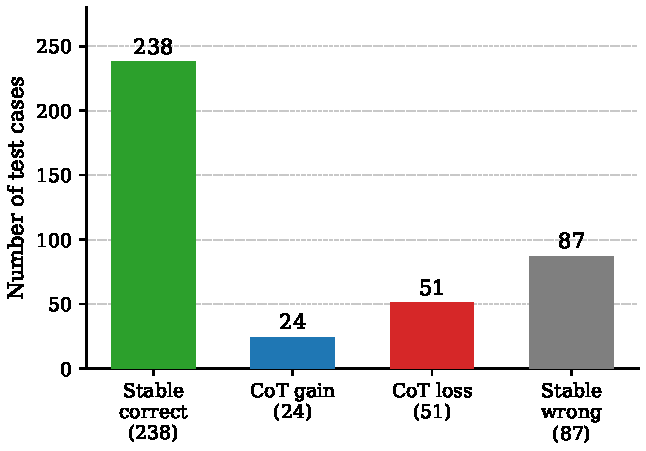
\includegraphics[width=0.55\textwidth]{pictures/figures/fig_cot_flip.pdf}
\caption{Flip analysis for Config~CD+Q+ITC relative to Config~CD+Q.
         Of 400 test cases, chain-of-thought breaks 50 previously correct
         predictions while recovering only 24 previously incorrect ones,
         for a net change of $-26$ cases.}
\label{fig:cot-flip}
\end{figure}

Table~\ref{tab:cot-case-studies} illustrates four representative losses. In
each case, Config~CD+Q produces the value accepted by the benchmark, and the
reasoning step overrides it with a linguistically natural alternative that the
benchmark does not accept.

\begin{table}[h]
\centering
\caption{Representative cases where chain-of-thought reasoning overrides a
correct Config~CD+Q prediction. Reasoning excerpts are taken verbatim from
stored reasoning traces.}
\label{tab:cot-case-studies}
\begin{tabular}{p{2.4cm} p{2.2cm} p{2.2cm} p{5.4cm}}
\toprule
Parameter & CD+Q & CoT & Reasoning excerpt \\
\midrule
\texttt{discount\_rate}
    & \texttt{0.1} $\checkmark$
    & \texttt{10.0} $\times$
    & ``The discount rate is in percentage form.
      Extracted arguments: discount\_rate = 10'' \\[4pt]
\texttt{fuel\_type}
    & \texttt{'gas'} $\checkmark$
    & \texttt{'gasoline'} $\times$
    & ``Gasoline would be the fuel type'' \\[4pt]
\texttt{duration}
    & \texttt{'2 weeks'} $\checkmark$
    & \texttt{'last 2 weeks'} $\times$
    & ``The duration is `last 2 weeks', which
      needs to be preserved exactly as a string'' \\[4pt]
\texttt{start\_date}
    & \texttt{'01/01/2021'} $\checkmark$
    & \texttt{'2021-01-01'} $\times$
    & ``start\_date: '2021-01-01'
      (assuming ISO 8601 format)'' \\
\bottomrule
\end{tabular}
\end{table}

Three mechanisms account for this pattern. First, the reasoning step introduces
drift: the model interprets the instruction to reason step by step as licence to
produce derivations and justification paragraphs before the extraction step,
consuming tokens without supplying useful information. Second, values committed
in the reasoning text act as a prior for the subsequent guided extraction: once
the reasoning block contains \texttt{discount\_rate = 10}, the guided step
inherits that value rather than re-evaluating it. Third, the model normalises
values toward linguistically standard forms. The benchmark's ground truth
encodes specific conventions, often arbitrary ones (abbreviations over full
words, decimal fractions for percentages, particular date formats), that
reasoning moves the model away from rather than toward. Config~CD+Q's one-step
guided decode produces the expected convention without verbalising it;
verbalising the reasoning surfaces the model's preferred form, which
consistently differs from the benchmark's.

The result extends the finding from Config~PE: the residual failure rate after
constrained decoding is caused by a mismatch between the model's priors and the
benchmark's labels, and interventions that make reasoning explicit exacerbate
this mismatch.

\subsection{Retrieval-Augmented Generation}

In all preceding configurations, each test case is provided with the exact
function definition required to answer it. Config~CD+Q+RAG replaces this oracle
provision with a retrieval step. All 370 unique function signatures from the
\texttt{simple\_python} category are embedded using
\texttt{sentence-transformers/all-MiniLM-L6-v2} and indexed with FAISS. At
inference time, the query is embedded and the top-5 most similar functions are
retrieved as candidates; the model must select the correct function from these
candidates and extract its arguments~\cite{lewis2020retrieval}. The result is
47.75\% accuracy (191/400), a decrease of 24~pp relative to Config~CD+Q.

The retrieval component achieves recall@5 of 97.2\% (389/400): the correct
function is present among the 5 retrieved candidates in 389 of 400 test cases.
The 11 retrieval failures occur on domain-ambiguous functions whose names share
little lexical overlap with the query (e.g., \texttt{calculate\_density},
\texttt{recipe\_search}, \texttt{sentiment\_analysis}). Retrieval quality is
therefore not the primary cause of the accuracy decrease.

The failure distribution identifies where accuracy is lost. Of the 400 test
cases, 264 (66.0\%) produce output identical to Config~CD+Q, indicating that
the additional candidates have no effect on these cases. In 128 cases (32.0\%),
the model selects a wrong function from the retrieved candidates. In 8 cases
(2.0\%), the correct function is selected but with incorrect argument values.
The dominant failure mode is function disambiguation. When a query for triangle
area retrieves \texttt{calculate\_triangle\_area}, \texttt{calculate\_area}, and
\texttt{calc\_area\_triangle} as candidates, the model selects a generic variant
in the majority of cases. Similar patterns are observed for mathematical
synonyms (\texttt{algebra.quadratic\_roots} vs.\ \texttt{solve\_quadratic\_equation})
and namespace variants (\texttt{geometry.circumference} vs.\
\texttt{calculate\_circumference}).

The result establishes that the bottleneck in a RAG-based tool-calling pipeline
for a 7B model is not retrieval quality but candidate discrimination. A
recall@5 of 97.2\% is sufficient for the retrieval component; the model lacks
the capacity to reliably distinguish among semantically similar candidate
functions once they are retrieved. Fig.~\ref{fig:rag-breakdown} summarises
the failure distribution across the 209 incorrect predictions.

\begin{figure}[htbp]
\centering
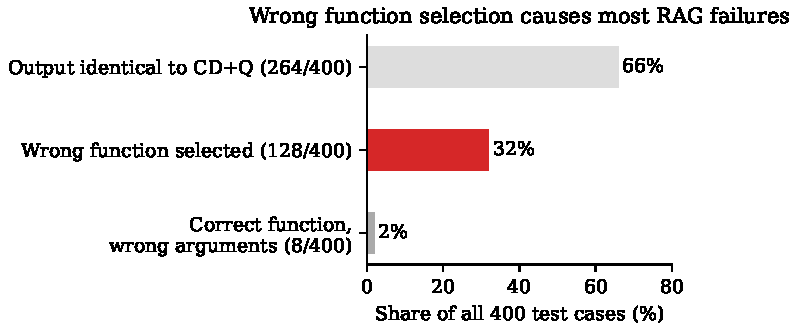
\includegraphics[width=0.55\textwidth]{pictures/figures/fig_rag_breakdown.pdf}
\caption{Failure breakdown for Config~CD+Q+RAG (209 incorrect predictions
         out of 400 test cases). The dominant failure mode is wrong function
         selection (32\%), not retrieval miss or argument extraction error.}
\label{fig:rag-breakdown}
\end{figure}

\section{Training-Based Methods}

\subsection{LoRA Fine-Tuning}

A LoRA adapter is trained on the Salesforce \texttt{xlam-function-calling-60k}
dataset~\cite{zhang2024xlam}, using 54{,}000 training examples and 6{,}000
validation examples. The
base model is \texttt{Qwen/Qwen2.5-7B-Instruct}, trained for 2 epochs with
LoRA rank~16 in bfloat16~\cite{hu2022lora}. The adapter is merged into the
base weights by linear interpolation before evaluation, producing a single
merged model at full bfloat16 precision.

Without constrained decoding (Config~FT-only), the fine-tuned model achieves
13.75\% accuracy (55/400), an improvement of 12.25~pp over the unguided
baseline Config~B (1.5\%). Fine-tuning on a function-calling corpus teaches the
model that tool-calling responses should be structured: parseable, single-object
JSON is produced in more cases than by the base model. The 12.25~pp gain
confirms that the training signal is meaningful and that the xlam examples
contain sufficient format regularity for format learning to occur.

The xlam dataset encodes assistant-turn responses as Python call syntax
(\texttt{func(arg=value, ...)}). This convention differs from the
evaluation pipeline, which expects a JSON argument object
(\texttt{\{"arg": value\}}). The format mismatch between the training
distribution and the evaluation format is the primary limitation of this
configuration, and its effect on the combined pipeline is examined in
Section~\ref{sec:combined-configs}.

\section{Combined Configurations}
\label{sec:combined-configs}

Config~CD+FT combines constrained decoding with the LoRA-merged model. The
result is 69.75\% accuracy (279/400), a regression of 3~pp relative to
Config~CD without fine-tuning. The combined configuration underperforms the
no-fine-tuning baseline.

The regression is attributed to the training format mismatch. Constrained
decoding enforces the surface format: every output is a valid JSON object
conforming to the function schema. However, the argument value predictions
remain biased toward the conventions of the training data. Since xlam encodes
argument values as part of Python call syntax, the fine-tuned model's weights
encode this convention. When constrained decoding forces the output to be valid
JSON, the value-level predictions are pulled toward xlam conventions rather than
the BFCL ground truth. A secondary contributing factor is the composition of
the training set: 52.6\% of xlam examples contain multiple function calls per
query, while the \texttt{simple\_python} category is exclusively single-call.
This distribution mismatch may shift the model's prior toward multi-call
patterns in contexts where a single call is required.

The gap between Config~FT-only (13.75\%) and Config~CD+FT (69.75\%) confirms
that constrained decoding remains the dominant contributor to accuracy even
after fine-tuning: removing it reduces accuracy by 56~pp. The two techniques
are complementary, but fine-tuning on a misaligned training distribution does
not improve on the CD baseline because the learned value conventions do not
match those of the evaluation benchmark.

\subsection{Format-Aligned Fine-Tuning}

The format mismatch identified in Config~CD+FT is addressed by rewriting
the training data preprocessor to produce assistant-turn responses that
match the inference pipeline's argument extraction prompt exactly.
Two variants are evaluated: Config~FT-aligned-ng, which applies the
format-aligned adapter without constrained decoding, and
Config~CD+FT-aligned, which combines the adapter with the full
constrained decoding pipeline.

Config~FT-aligned-ng achieves 13.25\% accuracy (53/400), a decrease of
0.5~pp relative to Config~FT-only. The format-aligned training objective
optimises for JSON-only argument extraction and omits the function name
from the assistant turn, as required by the guided inference pipeline.
The unguided evaluator must recover the function name from the raw output;
because the training format no longer produces it, the unguided pass rate
decreases. Format alignment improves the guided inference path at the cost
of degrading the unguided path.

Fig.~\ref{fig:lora-training-loss} shows the training loss for both adapters.
Both runs use identical hyperparameters and converge to similar final losses
(v1: 0.203, v2: 0.229 at step 6750), confirming that the v1 regression is
not a training failure. The difference in BFCL accuracy (69.75\% vs.\
76.75\%) is attributable to the training format, not to convergence quality.

\begin{figure}[htbp]
\centering
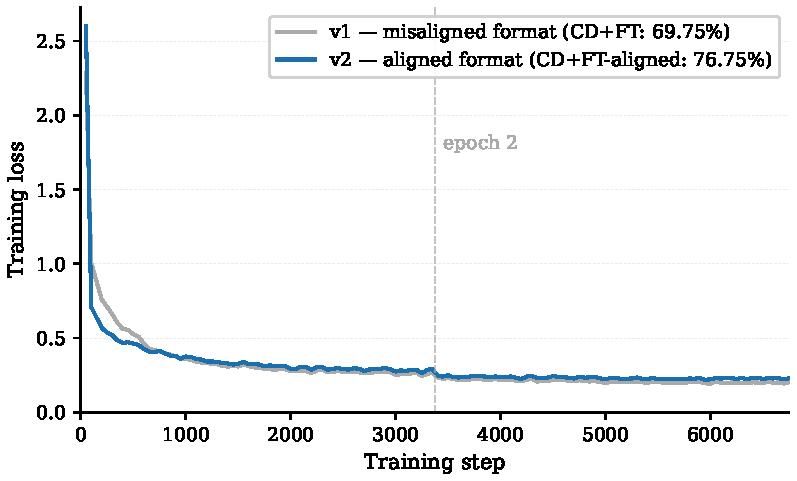
\includegraphics[width=0.65\textwidth]{pictures/figures/fig_lora_training_loss.pdf}
\caption{Training loss for the misaligned (v1) and format-aligned (v2) LoRA
         adapters over 6{,}750 steps (2 epochs on 54{,}000 xlam examples).
         Both runs converge to comparable loss values; the 7.0~pp accuracy
         difference between Config~CD+FT and Config~CD+FT-aligned is caused
         by the training output format, not by training quality.}
\label{fig:lora-training-loss}
\end{figure}

Config~CD+FT-aligned achieves 76.75\% accuracy (307/400), an improvement
of 4.0~pp over Config~CD and 7.0~pp over Config~CD+FT. This is the highest
accuracy observed across all configurations. Format-aligned fine-tuning
breaks the no-training ceiling of 72.75\% established by Config~CD.

The 23.25\% failure rate that remains under Config~CD+FT-aligned follows
the same taxonomy as Config~CD: optional parameter defaults, numeric
precision, string format conventions, and enum value mismatches. The xlam
training examples do not supply argument values that match BFCL ground
truth labels closely enough to eliminate these failure categories. The
4.0~pp gain over Config~CD reflects a reduction in error frequency, not
the introduction of a new success mechanism.

Table~\ref{tab:full-ablation} presents all ten configurations ordered
by accuracy, and Fig.~\ref{fig:bfcl-ablation} shows the same data as
a bar chart with frontier reference lines.

\begin{table}[h]
\centering
\caption{BFCL v4 simple\_python AST accuracy across all ten configurations.
         $\Delta$ is relative to Config~CD (72.75\%).}
\label{tab:full-ablation}
\begin{tabular}{llrr}
\toprule
Config & Technique & Accuracy (↑) & $\Delta$ vs CD \\
\midrule
B             & Raw baseline                & 1.50\%  & $-71.25$~pp \\
FT-aligned-ng & Format-aligned LoRA, no CD & 13.25\% & $-59.50$~pp \\
FT-only       & LoRA, no CD                & 13.75\% & $-59.00$~pp \\
CD+Q+RAG      & CD + AWQ + RAG top-5       & 47.75\% & $-25.00$~pp \\
CD+Q+ITC      & CD + AWQ + CoT             & 65.50\% & $-7.25$~pp  \\
CD+FT         & CD + LoRA (misaligned)     & 69.75\% & $-3.00$~pp  \\
PE            & CD + few-shot              & 70.25\% & $-2.50$~pp  \\
CD+Q          & CD + AWQ INT4              & 72.25\% & $-0.50$~pp  \\
CD            & Constrained decoding       & 72.75\% & --          \\
CD+FT-aligned & CD + format-aligned LoRA   & \textbf{76.75\%} & $\mathbf{+4.00}$~pp \\
\bottomrule
\end{tabular}
\end{table}

\begin{figure}[htbp]
\centering
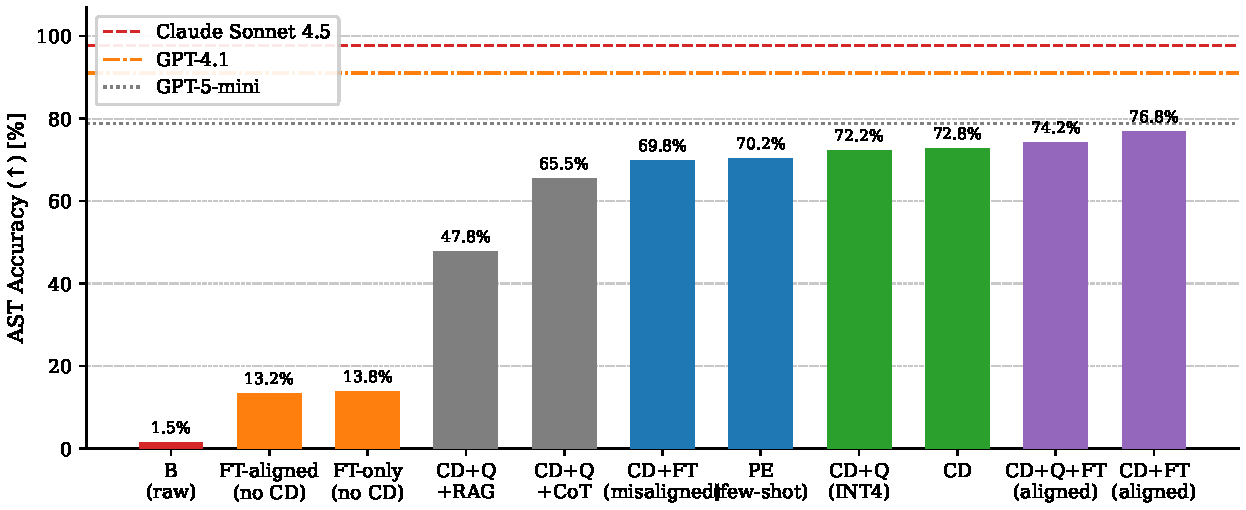
\includegraphics[width=\textwidth]{pictures/figures/fig_bfcl_ablation.pdf}
\caption{BFCL v4 simple\_python AST accuracy for all ten configurations.
         Dashed reference lines show Gemini~3 Pro (79.58\%),
         Claude Opus~4.5 (76.83\%), and GPT-4.1 (72.67\%).
         Config~CD+FT-aligned (purple) is the only configuration to
         exceed the no-training ceiling established by Config~CD.}
\label{fig:bfcl-ablation}
\end{figure}

\section{Comparison with Frontier Models}

Table~\ref{tab:frontier-comparison} compares the Qwen~2.5 7B-Instruct results against frontier models, using official scores from the BFCL~v4 leaderboard\footnote{\url{https://gorilla.cs.berkeley.edu/leaderboard.html}, accessed April 2026.} for the Non-Live Simple AST category.

\begin{table}[h]
\centering
\caption{BFCL v4 Simple Function AST accuracy: Qwen~2.5 7B with constrained decoding vs.\ frontier models (official leaderboard scores).}
\label{tab:frontier-comparison}
\begin{tabular}{llr}
\toprule
Model & Type & Accuracy (↑) \\
\midrule
Gemini 3 Pro          & Frontier & 79.58\% \\
Claude Opus 4.5       & Frontier & 76.83\% \\
GPT-4.1-mini          & Frontier & 73.33\% \\
GPT-4.1               & Frontier & 72.67\% \\
Claude Sonnet 4.5     & Frontier & 72.58\% \\
Claude Haiku 4.5      & Frontier & 71.00\% \\
GPT-5-mini            & Frontier & 59.92\% \\
\midrule
Qwen 2.5 7B + CD+FT-aligned & SLM (ours) & \textbf{76.75\%} \\
Qwen 2.5 7B + CD            & SLM (ours) & 72.75\% \\
Qwen 2.5 7B + PE            & SLM (ours) & 70.25\% \\
Qwen 2.5 7B (raw)           & SLM (ours) & 1.50\%  \\
\bottomrule
\end{tabular}
\end{table}

\begin{figure}[htbp]
\centering
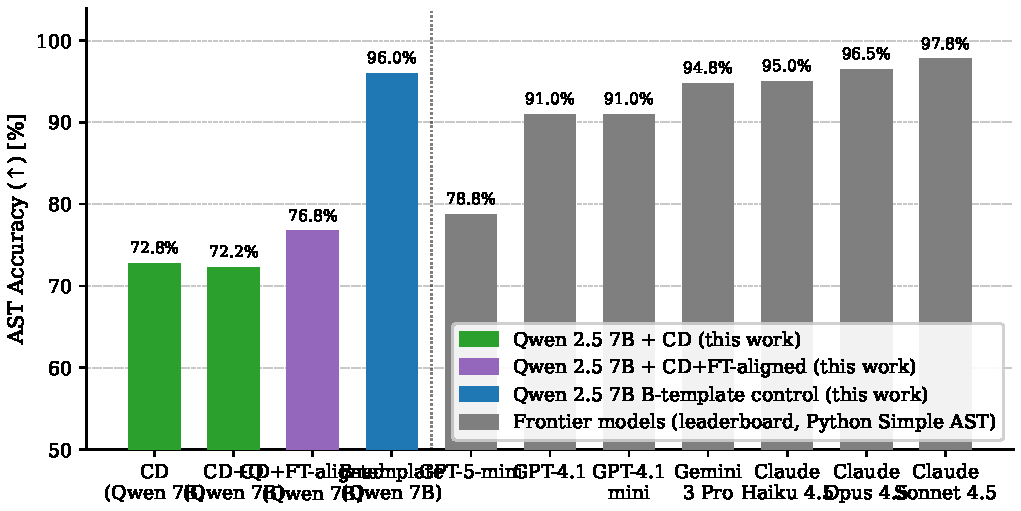
\includegraphics[width=\textwidth]{pictures/figures/fig_frontier_comparison.pdf}
\caption{BFCL v4 simple\_python AST accuracy for Qwen~2.5 7B configurations
         (this work) vs.\ frontier models from the official leaderboard
         (accessed April 2026). Config~CD+FT-aligned reaches 76.75\%,
         within 0.08~pp of Claude Opus~4.5 (76.83\%).}
\label{fig:frontier-comparison}
\end{figure}

\noindent Fig.~\ref{fig:frontier-comparison} and
Table~\ref{tab:frontier-comparison} compare the Qwen~2.5 7B results against
the leaderboard. Qwen~2.5 7B-Instruct with constrained decoding alone
(72.75\%) matches or exceeds several frontier models on Simple Function
accuracy, including GPT-4.1 (72.67\%), Claude Sonnet~4.5 (72.58\%), and
Claude Haiku~4.5 (71.00\%). With format-aligned fine-tuning,
Config~CD+FT-aligned reaches 76.75\%, within 0.08~pp of Claude Opus~4.5
(76.83\%). The gap to the best frontier model (Gemini~3 Pro at 79.58\%)
is 2.83 percentage points.

This suggests that for single-call function calling with a well-defined schema, constrained decoding on a 7B model closes the gap to frontier-level performance. The remaining gap is driven by argument value accuracy, not format compliance or function selection---the same bottleneck that limits the frontier models themselves.

However, this result requires careful interpretation. The simple\_python category is the least demanding BFCL scenario: single-turn, single-function calls with no selection ambiguity (one candidate function per test case). Both constrained decoding and frontier models' native tool-calling APIs guarantee valid JSON and valid function names, levelling the playing field on format compliance. The only differentiator is argument value accuracy, where a 7B model can be competitive on straightforward lookups.

Frontier models distinguish themselves on harder tasks. Their BFCL overall
scores, which weight multi-turn (30\%) and agentic tasks (40\%), remain
substantially higher than what an SLM would likely achieve on those
categories. Claude Opus~4.5 maintains 77.47\% overall, while GPT-4.1
drops to 53.96\%, indicating that even among frontier models, simple
function calling does not predict general agentic capability. The
multi-step evaluation in Section~\ref{sec:tau-bench} quantifies where
the SLM--frontier gap re-emerges.

\section{Agentic Evaluation}
\label{sec:tau-bench}

Single-call tool accuracy measures one dimension of agent capability.
The $\tau$-bench retail benchmark evaluates end-to-end task completion
across multi-turn interactions, where the model must select tools, observe
results, and iterate until a retail service task is
resolved~\cite{taubench2024}. Config~CD is evaluated on the retail domain
test split (115 tasks) to establish the agentic baseline.

Three full runs are completed to account for user simulator variance.
Pass rates of 4.35\%, 5.22\%, and 3.48\% are observed for runs~1, 2,
and~3 respectively, with a mean of 4.35\% (5/115). The user simulator
(Qwen~2.5 7B on the same vLLM instance) generates stochastic responses
despite the model running at temperature~0.0, producing the observed
inter-run variance. At $n=115$ binary tasks the standard error is
approximately 1.9~pp; the observed range of 3.5--5.2\% is within this
noise band.

Scoring is binary: a task passes only if the final database state exactly
matches the ground truth at the end of the interaction. Partial completion
yields reward~0.0. This criterion reflects the operational requirement
that retail service tasks must be resolved completely; partial execution
has no customer-facing value.

Table~\ref{tab:bfcl-vs-tau} places the single-call and multi-step results
side by side.

\begin{table}[h]
\centering
\caption{Single-call accuracy (BFCL) vs.\ multi-step pass rate
         ($\tau$-bench) for Config~CD on Qwen~2.5 7B-Instruct.}
\label{tab:bfcl-vs-tau}
\begin{tabular}{llr}
\toprule
Benchmark & Setting & Pass rate (↑) \\
\midrule
BFCL simple\_python & Single call, 1 turn     & 72.75\% \\
$\tau$-bench retail & Multi-step, 5--15 turns & 4.35\%  \\
\bottomrule
\end{tabular}
\end{table}

The 68.4~pp gap between the two benchmarks is the central result of this
section. A model that generates individually valid tool calls 72.75\% of
the time achieves end-to-end task success only 4.35\% of the time on the
retail domain.

Four failure categories are identified by trajectory inspection. State
drift is the most frequent: the model does not track which items have been
modified across turns when a request involves multiple sub-tasks. Premature
termination is observed when the model calls \texttt{finish} before all
sub-tasks are resolved, particularly on multi-item requests. Tool parameter
errors persist despite Config~CD achieving near-perfect function selection
on BFCL, because $\tau$-bench tools accept free-form string identifiers
that constrained decoding does not validate. Context management failures
are also observed in tasks with long conversation histories, where earlier
tool call results are displaced from the model's working context.

The 4.35\% pass rate on $\tau$-bench establishes the agentic baseline for
Config~CD on the retail domain. The 68.4~pp gap quantifies the boundary
separating single-call function calling from reliable multi-step agentic
task completion.

% -----------------------------------------------------------------------
% PENDING: Model-Size Scaling (Jobs 28341336--28341341)
% Configs B and CD across 0.5B, 1.5B, 3B
% -----------------------------------------------------------------------
\section{Model-Size Scaling}
\label{sec:model-size}

% TODO: results table (B and CD accuracy vs model size: 0.5B, 1.5B, 3B, 7B)
% TODO: analysis of how the CD gain scales with model size

% -----------------------------------------------------------------------
% PENDING: Extended BFCL Categories (Jobs 28341342--28341347)
% multiple_function and parallel_function, 7B-AWQ, B+CD+CD+Q
% -----------------------------------------------------------------------
\section{Extended Function-Calling Categories}
\label{sec:bfcl-extended}

% TODO: multiple_function and parallel_function results table
% TODO: analysis of how candidate disambiguation affects accuracy

% -----------------------------------------------------------------------
% PENDING: Quantized Fine-Tuned Model (Jobs 28341348--28341349)
% CD+Q+FT: AWQ quantize merged format-aligned LoRA + BFCL eval
% -----------------------------------------------------------------------
\section{Quantized Fine-Tuning}
\label{sec:cdqft}

% TODO: CD+Q+FT result and comparison to CD+FT-aligned and CD+Q
